\begin{frame} \frametitle{ Hybrid System Simulation }
	\vspace{-5pt}
	\begin{block}{Continuous Behaviour}
		\begin{myitemize}
			\item Continuous behaviour is captured using \textbf{ODEs}.
			\item Use \textbf{numerical methods} to solve ODEs.
			\begin{itemize}
				\item \textbf{Runge-Kutta (RK45)} is dominantly used
				\item Taylor, Euler, QSS, etc.
			\end{itemize}
		\end{myitemize}
	\end{block}
	
	\begin{block}{Discrete Behaviour}
		\begin{myitemize}
			\item Discrete behaviour is captured as discontinuity.
			\item Use \textbf{zero-crossing algorithms} to detect discontinuous points.
			\begin{itemize}
				\item {Bracket method} is used by Simulink.
				\item {Bisection method} is used by OpenModelica.
			\end{itemize}
		\end{myitemize}
	\end{block}
\end{frame}


\begin{frame} \frametitle{ Simulation Requirements }
	\vspace{-5pt}
	\begin{myitemize}
		\item Cyber-Physical Systems (CPSs) are safety-critical hybrid systems
		\item These require precise simulation for validation
	\end{myitemize}
	
	\begin{block}{ Requirements }
		\begin{myitemize}
			\item \textbf{Bounded local truncation error (LTE)} in solving ODEs.
			\item \textbf{Guaranteed zero-crossing detection (ZCD)}. This should deal with: 
			\begin{itemize}
				\item Even number of zero-crossings
				\item Falling into complex plane 
				\item Touching the zero-line
			\end{itemize}
		\end{myitemize}
	\end{block}
	
	\begin{figure}
		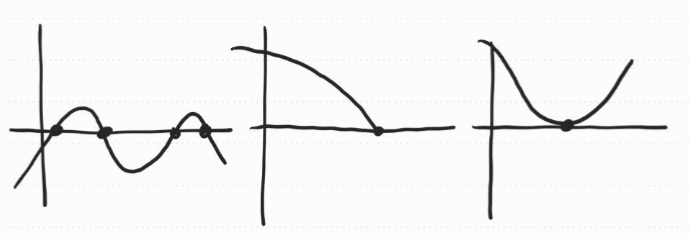
\includegraphics[width=0.6\textwidth]{./fig/zero-crossings.png}
	\end{figure}
	
\end{frame}

\begin{frame} \frametitle{RK45 (Fehlberg)}
	\vspace{-5pt}
	\begin{block}{Basic Idea}
		\begin{enumerate}
			\item Includes an adaptive step size algorithm
			\item $LTE = RK5(\Delta t) - RK4(\Delta t)$
			\item Increase/decrease the step size $\Delta t$ to control LTE
			\item Bounded LTE constraint: $|LTE| < tol$
		\end{enumerate}
	\end{block}
	
	\begin{block}{Limitation}
		\begin{enumerate}
			\item RK45 alone cannot do ZCD.
			\item Using root-finding algorithms with RK45 is theoretically possible, but will be extremely slow and can still miss ZCD.
		\end{enumerate}
	\end{block}
	\centering
\end{frame}

\begin{frame} \frametitle{Bracket/Bisection Methods}
	\vspace{-5pt}
	\begin{block}{Basic Idea}
		\begin{enumerate}
			\item Iterative approaches based on sign-change detection.
			\item Can be used with RK45.
		\end{enumerate}
	\end{block}
	
	\begin{block}{Limitation}
		\begin{enumerate}
			\item There must be a sign-change.
			\item Cannot handle challenging situations: 
			\begin{itemize}
				\item even number of zero-crossings
				\item complex plane
				\item touching the zero-line
			\end{itemize}
			\item Zero-crossing detection cannot be guaranteed.
		\end{enumerate}
	\end{block}
	\centering
\end{frame}

\begin{frame} \frametitle{ MQSS Methods }
	\vspace{-5pt}
	\begin{block}{Basic Idea}
		\begin{enumerate}
			\item In order to ensure zero-crossing detection, we proposed MQSS.
			\item Approximate each variable, and solve the guard.
			\item Using QSS-1 and QSS-2, two time solution $t1$ and $t2$ can be calculated.
			\item Ensure $|t1 - t2| < ttol$ by controlling $\Delta q$.
		\end{enumerate}
	\end{block}
	
	\begin{block}{Limitation}
		\begin{myitemize}
			\item Guard conditions have to be univariate
			\item Possibly slow solving due to many iterations needed to reach $|t1 - t2| < ttol$
			\item At stationary point $\dot{x} = 0$, there is no solution for $t$. Thus, the algorithm terminates unsuccessfully.
		\end{myitemize}
	\end{block}
	\centering
\end{frame}

\begin{frame} \frametitle{MQSS Finding the next time step }
	\centering
	\begin{figure} 
		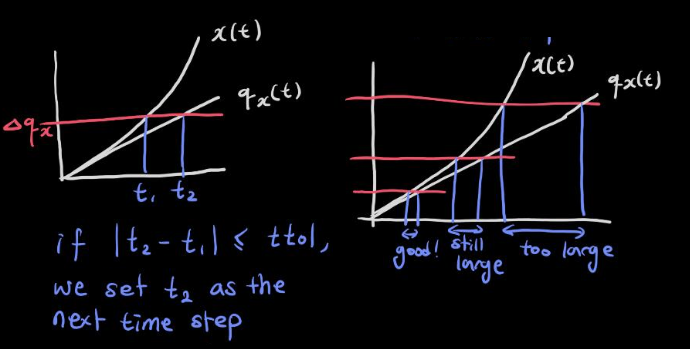
\includegraphics[width=1\textwidth]{./fig/dq1.png}
	\end{figure}
\end{frame}



\begin{frame} \frametitle{ Problem Statement }
	\begin{enumerate}
		\item Typical CPS models include multivariate nonlinear ODEs and guards.
		\item Precise simulation requires: 
			\begin{itemize}
			\item Bounded LTE
			\item Guarnateed ZCD
			\end{itemize}
		\item RK45 with Bracket/Bisection methods cannot guarantee ZCD.
		\item Recently proposed MQSS is accurate and can guarantee ZCD.
		\item However, MQSS has major limitations:
			\begin{itemize}
				\item Only allows univariate guards
				\item Simulation execution is slow
				\item Adaptive step size algorithm fails at stationary points
			\end{itemize}
		\item Thus, MQSS cannot simulate every CPS model.
		\item We need to overcome such limitations.
	\end{enumerate}
	
\end{frame}

\begin{frame} \frametitle{Contributions}
	\begin{myitemize}
		\item A new extension to HIOA, called HIOA/PD ( Hybrid Input Output Automata / Precomputed Differentiations )
		\item Compositional semantics including smooth-token exchange.
		\item A new algorithm for calculating the next time step.
		\item Comparison with existing methods.
	\end{myitemize}
\end{frame}

\begin{frame}[c] \frametitle{ Proposing idea brief description }

	\begin{enumerate}
		\item Convert the Simulink/Stateflow model into HIOA.
		\item This HIOA includes ODEs ($f$), update functions ($h$), and guards ($g$). These are all expressed as a function.
		\item By taking advantage of Sympy, precompute the differentiation for $f$, $h$, and $g$, up to the $\alpha$.
		\item Capture them in a new structure called HIOA/PD.
		\item Add smooth-tokens to allow exchange of derivative values between HIOA.
		\item For each continuous variable, we can obtain up to $n$th derivative value. Thus, we can approximate with $n$th order Taylor polynomials.
		\item Similarly, we compute I/O variables smooth-tokens.
		\item Finally, we can approximate $g$ using $n$th order Taylor polynomials. The only variable is $t$, so we can be solve it for $t$. Also, based on $g$, we set $\Delta q$.
	\end{enumerate}

\end{frame}

\begin{frame}[c] \frametitle{ Key Points }

	\begin{myitemize}
		\item We can guarantee that we always get at least one positive real root. This ensures that we always find delta values.
		\item We can guarantee that the found zero-crossing is always the first one. This ensures that we always correctly find zero-crossing.
		\item We can guarantee that the found solution $t$ is within the valid interval, which satisfies bounded LTE.
	\end{myitemize}

\end{frame}

\begin{frame}[c] \frametitle{ HIOA/PD Definition }
	\vspace{-5pt}
	\begin{block}{}
		$\mathcal{H} = \langle \alpha, L, X, V, O, Init, Inv, f, h, E, G, R\rangle $
		\begin{itemize}
		\item $\alpha \in \mathbb{N}_{\geq 1}$ is the maximum derivative order.
		\item $L = \{l_{0},\ldots,l_{n}\}$ a set of discrete locations.
		\item $X$ is a finite collection of continuous variable smooth-tokens. A smooth-token $x \in X$ is a sequence, $x = [ x^{(0)}, x^{(1)}, ..., x^{(\alpha)} ] $, where $x^{(n)} \in \mathbb{R}$ is $n$th derivative value. The domain of $X$ is $\mathbf{X} = \mathbb{R}^{n \times (\alpha + 1)}$, where $n$ is the number of continuous variables.
		\item $V$ is a finite collection of input variable smooth-tokens. For $v \in V$, $v$ is a sequence up to $\alpha$th derivative. The domain of $V$ is $\mathbf{V}$.
		\item $O$ is a finite collection of output variable smooth-tokens. For $o \in O$, $o$ is a sequence up to $\alpha$th derivative. The domain of $O$ is $\mathbf{O}$.
		\item $Init \subseteq \{l_0\} \times \mathbf{X} \times \mathbf{O}$.
		\item $Inv: \mathbf{L} \rightarrow 2^{\mathbf{X} \times \mathbf{V} }$
		\end{itemize}
	\end{block}
\end{frame}

\begin{frame}[c] \frametitle{ HIOA/PD Definition Cont. }
	\vspace{-5pt}
	\begin{block}{}
		\begin{itemize}
		
		\item $f : \mathbf{L} \times \mathbf{V} \times \mathbf{X} \times \mathbb{N}_{\geq 0,\leq \alpha} \rightarrow \mathbb{R}^{n}$ is a vector field for ODEs. E.g., 
		\begin{equation}
			f(l_0, V, X, 1) \myeq 
			\begin{bmatrix} 
				x^{(1)} \\
				y^{(1)} 
			\end{bmatrix}
			= 
			\begin{bmatrix} 
				\dot{x} \\
				\dot{y} 
			\end{bmatrix}
			=
			\begin{bmatrix}
				x \cos (y) \\
				x - y
			\end{bmatrix}
		\end{equation}
		\begin{equation}
			f(l_0, V, X, 2) \myeq 
			\begin{bmatrix} 
				x^{(2)} \\
				y^{(2)} 
			\end{bmatrix}
			= 
			\begin{bmatrix} 
				\ddot{x} \\
				\ddot{y} 
			\end{bmatrix}
			=
			\begin{bmatrix}
				-x \sin (y) \frac{dy}{dt} + \frac{dx}{dt} \cos (y) \\
				\frac{dx}{dt} - \frac{dy}{dt}
			\end{bmatrix}
		\end{equation}
		\item $h : \mathbf{L} \times \mathbf{X} \rightarrow \mathbf{O}$.
		\item $E \subset \mathbf{L} \times \mathbf{L} $ is a collection of discrete edges.
		\item $G : E \rightarrow 2^{\mathbf{X} \times \mathbf{V}}$ assigns to each
		  $e = (l, l') \in E$ a guard.
		\item
		  $R : E \times \mathbf{X} \times \mathbf{V} \rightarrow 2^{\mathbf{X} \times \mathbf{O}}$
		  assigns to each $e = (l,l') \in E$.
		\end{itemize}
	\end{block}
\end{frame}





